\documentclass[11pt]{article} % use larger type; default would be 10pt

\usepackage{graphicx} % support the \includegraphics command and options
\usepackage[margin=1.0in]{geometry}
\usepackage{amssymb}
\usepackage{amsmath}

\title{\textbf{An Improved Partitioned Element Method for Nonlinear Solid Mechanics}}
\author{M. M. Rashid, B. Giffin, S. Wopschall}
\date{}

\begin{document}
\maketitle


\begin{abstract}
We present an improved reformulation of the ``partitioned element method'' (PEM): a finite-element-like method in which shape functions are defined on arbitrary polygonal and polyhedral element domains. The method proceeds by partitioning an element into quadrature cells, and allowing the element's shape functions to vary according to a local polynomial defined within each of these cells, resulting in piece-wise polynomial shape functions which are discontinuous at quadrature cell boundaries. The polynomial coefficients defined in each cell are obtained by minimizing a quadratic functional which penalizes discontinuities in the shape functions (and their gradients) across all cell interfaces. Unlike the original method (presented in \cite{pem}) which is restricted to piece-wise linear approximants, the present formulation admits polynomials of arbitrary degree, leading directly to higher-order completeness of the shape functions, and improved convergence properties. Numerical results for two- and three-dimensional solid mechanics problems are presented, demonstrating the method's ability to overcome issues pertaining to non-convex elements and geometric degeneracies.
\end{abstract}

\section{Introduction}

Many recent developments in PEM are in need of an in-depth discussion following the original paper \cite{pem}. Most notably, the nature of how the shape functions are determined within an element is substantially changed. This paper seeks to elaborate on these differences; it does not address issues of computational geometry -- the partitioning of elements into quadrature cells.

\section{Formulation}

Central to the PEM is the idea that the domain $\Omega \subset \mathbb{R}^d$ is eponymously ``partitioned'' into a finite number of disjoint polytopal subsets, generically denoted $\omega_i \subset \Omega$, and more specifically referred to as verticies $v_i \in \mathcal{V}$ (0-topes), segments $s_i \in \mathcal{S}$ (1-topes), facets $f_i \in \mathcal{F}$ (2-topes), and cells $c_i \in \mathcal{C}$ (3-topes), whose union is $\Omega$.

\begin{figure} [!ht]
	\centering
	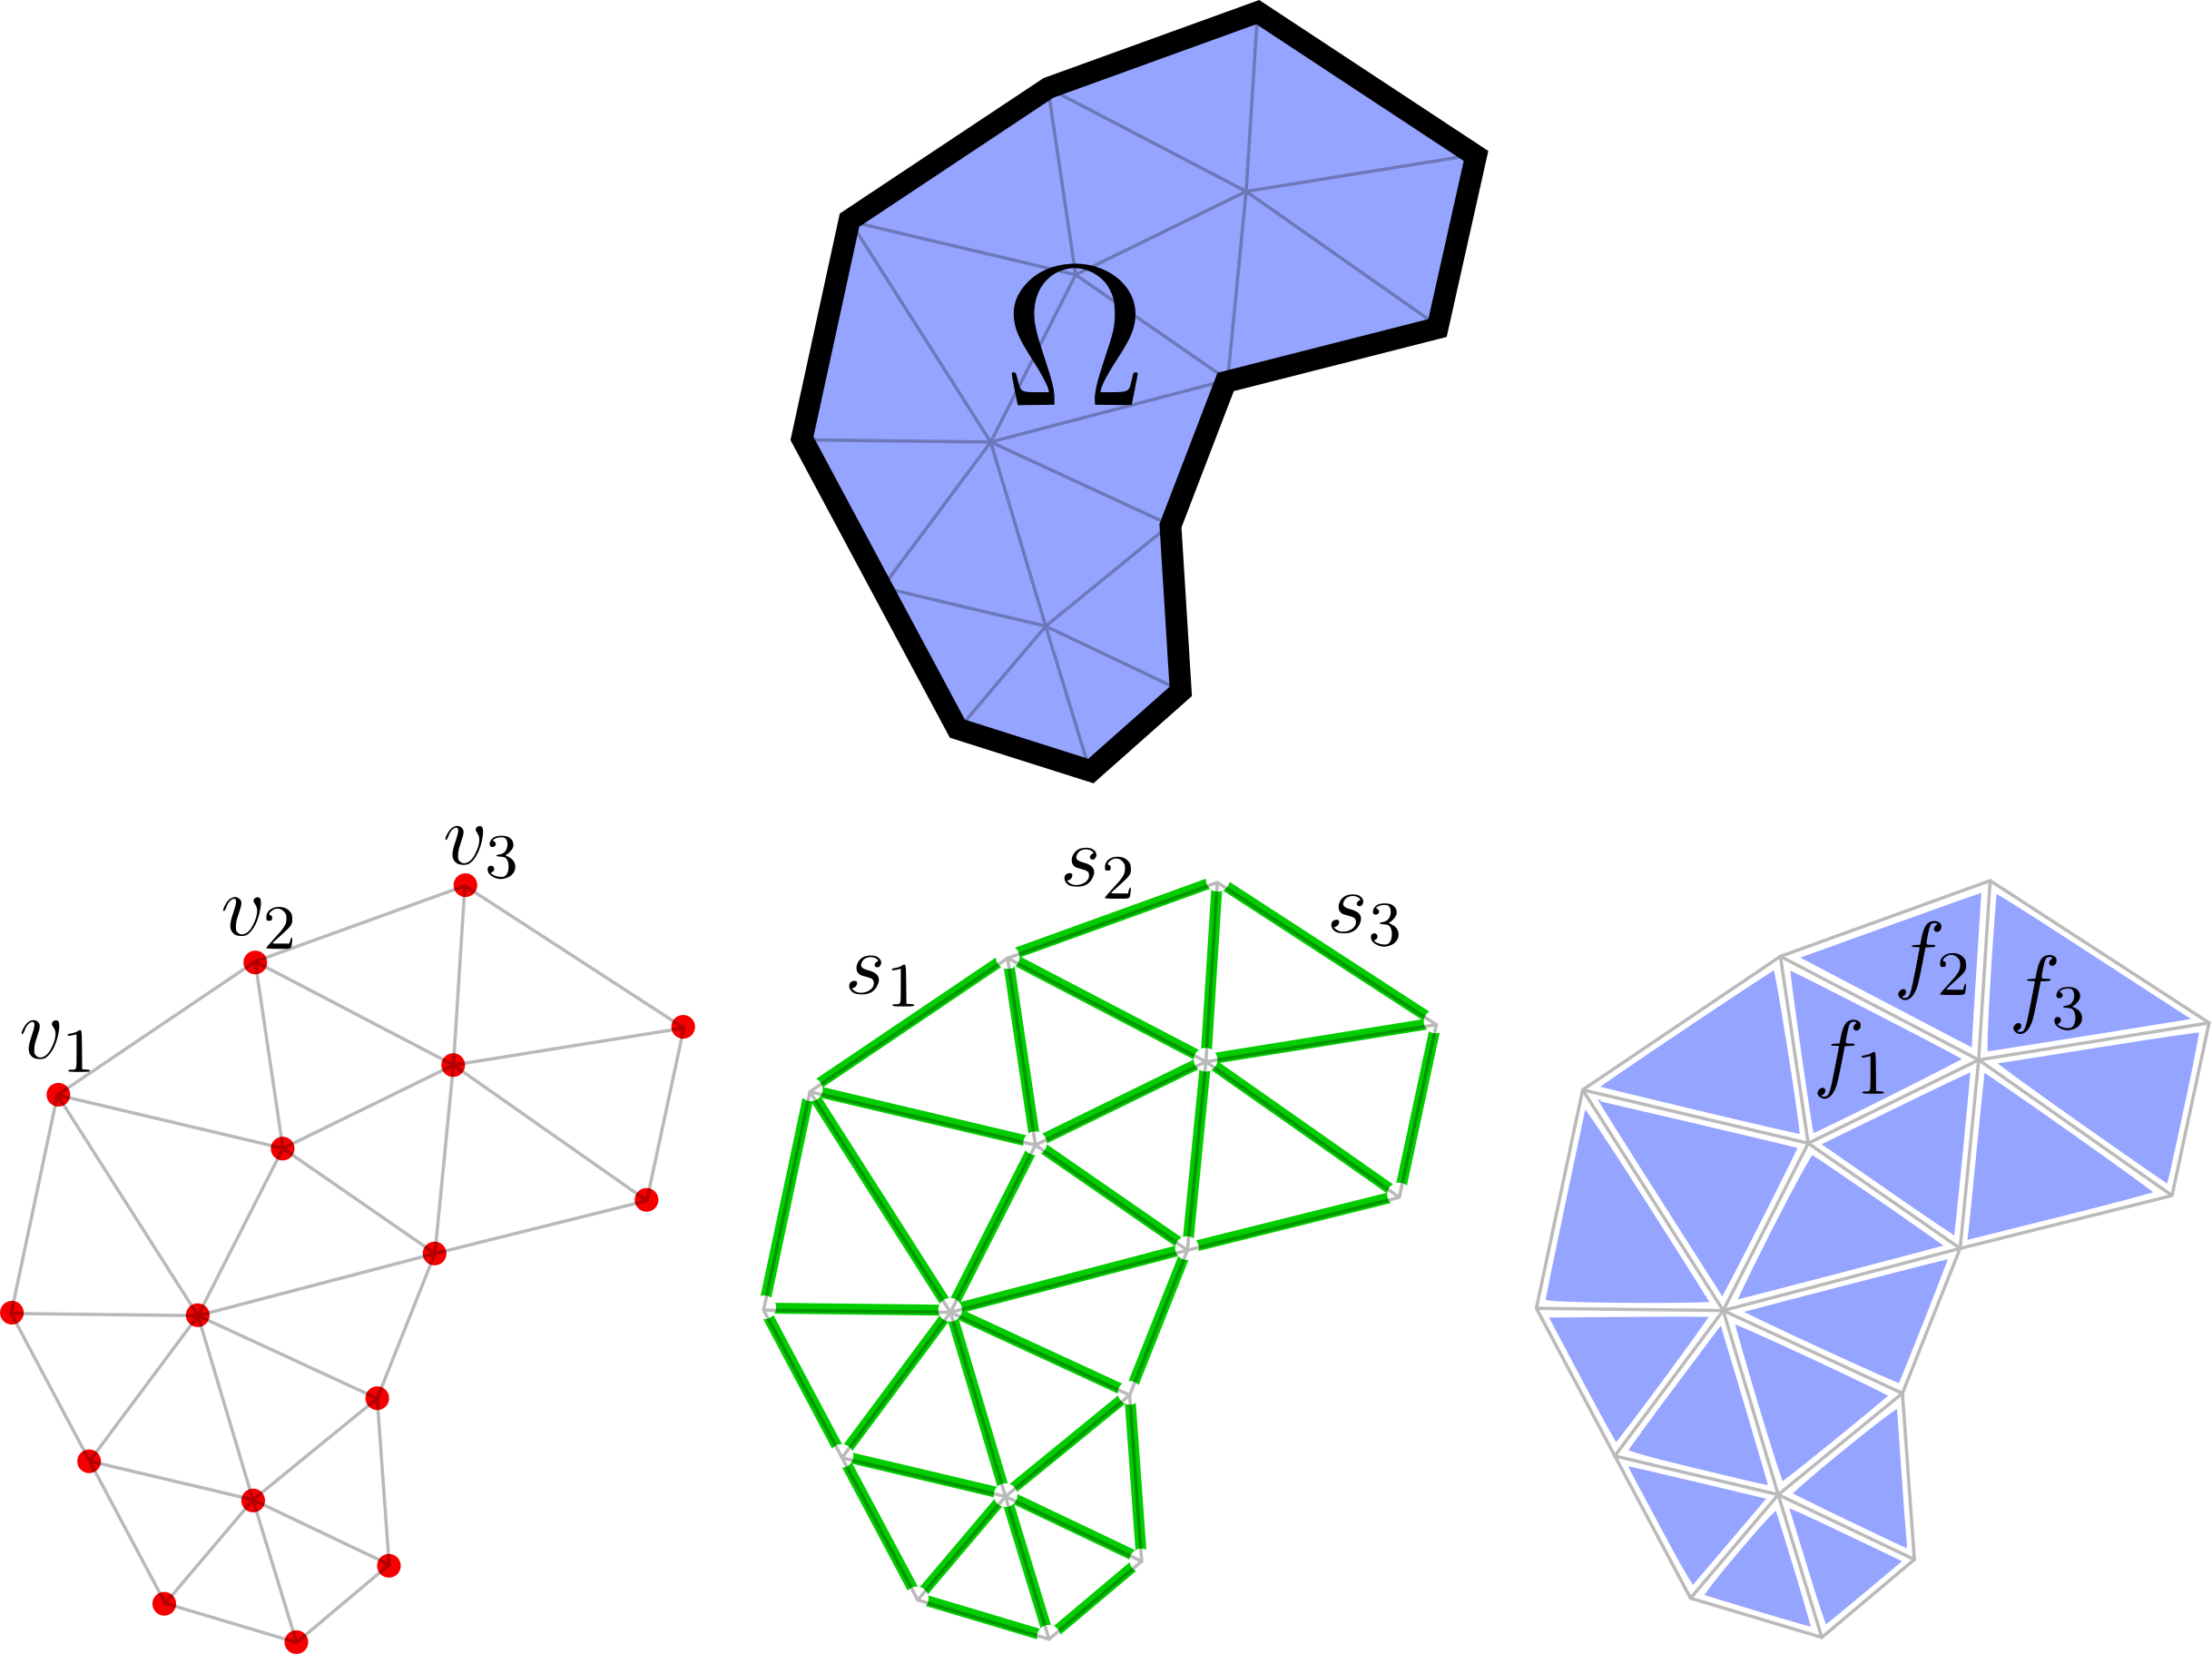
\includegraphics[width = 4.0in]{figures/partition.png}
	\caption{A representative domain $\Omega \subset \mathbb{R}^2$, and it's corresponding partition into verticies, segments, and facets.}
	\label{fig:partition}
\end{figure}

Given a partition of $\Omega$, we consider a number of additional set structures, which we shall refer to generically as ``elements,'' denoted $K_i$, and more specifically as $N_i$ (nodes), $E_i$ (edges), $F_i$ (faces), and $V_i$ (volumes). Nodes bear the primary degrees of freedom of the finite element problem at hand, and identify with individual verticies; edges identify a simply connected subset of segments and verticies, and are bounded by nodes; faces identify a simply connected subset of facets, segments, and verticies, and are bounded by edges; volumes identify a simply connected subset of cells, facets, segments, and verticies, and are bounded by faces. We require that every non-empty intersection between two elements be equal to the union of one or more ``sub''-elements, i.e. $K_i \cap K_j = \cup_k K_k \, \forall K_i \cap K_j \neq \emptyset$. Specifically, $V_i \cap V_j \forall i \neq j$ is the union of one or more faces/edges/nodes, $F_i \cap F_j \, \forall i \neq j$ is the union of one or more edges/nodes, and $E_i \cap E_j \, \forall i \neq j$ is a single node.

The space of functions under consideration in the PEM are those functions $u \in \mathcal{P}_k (\Omega)$, such that
\begin{equation}
	\mathcal{P}_k (\Omega) = \{ u : \, u|_{\omega} \in P_k (\omega) \, \forall \omega \subset \Omega \}.
\end{equation}
We denote $u|_{\omega}$ as the restriction of $u$ to the subset $\omega$, and $P_k (\omega)$ as the set of polynomials of maximal degree $k \geq 0$ defined on $\omega$. Any function $u \in \mathcal{P}_k (\Omega)$ is weakly differentiable, and well-defined on every generic subset $\omega \subset \Omega$.

The ultimate goal of the PEM is to construct a set of linear operators which map nodal values to edge values ($u|_{N_i} \mapsto u|_{E_i}$), edge values to face values ($u|_{E_i} \mapsto u|_{F_i}$), face values to volume values ($u|_{F_i} \mapsto u|_{V_i}$), and therefore, vicariously, nodal values to volume values ($u|_{N_i} \mapsto u|_{V_i}$).

Proceeding in sequence: for a given edge $E_i$ and known nodal values $u|_{N_j} \, \forall N_j \in E_i$, we wish to determine the corresponding values of $u$ defined on the set of all verticies and segments belonging to that edge (i.e. $u|_{v_j} \, \forall v_j \in E_i$ and $u|_{s_j} \forall s_j \in E_i$) such that the necessary and sufficient conditions for convergence of the finite element method are satisfied. These conditions are: stability, consistency, and completeness. For the moment, let us consider the space of PEM functions $u \in \mathcal{P}_1  (\Omega)$ (i.e. the space of piece-wise discontinuous polynomials of maximal degree 1.) In this setting, $u|_\omega \in P_1 (\omega) \, \forall \omega \in E_i$, meaning $u$ is defined independently on each $\omega$ as a linear polynomial:
\begin{equation}
	u|_\omega (\mathbf{x}) = c_\omega + \mathbf{g}_\omega \cdot \mathbf{x} \quad \forall \mathbf{x} \in \omega.
\end{equation}
We seek the polynomial coefficients $\{ c_\omega, \, \mathbf{g}_\omega \} \, \forall \omega \in E_i$ which are uniquely determined by the nodal values of the edge $u|_{N_j} \, \forall N_j \in E_i$.

In considering the space of functions $\mathcal{P}_1 (\Omega)$, we remark that any $u \in \mathcal{P}_1 (\Omega)$ will be a discontinuous function, in general. For the sake of stability, however, we should desire for $u$ to be ``minimally'' discontinuous, in some sense. Traditionally, this condition incorporates itself into the Weak Galerkin and Discontinuous Galerkin frameworks as a penalty term which promotes continuity of $u$. In like fashion, we will choose to pursue a penalty approach for the weak enforcement of continuity. Typical penalty strategies 

Additionally, we require (for the sake of completeness) that $u|_{E_i} \in P_1 (E_i)$ in the case where $u|_{N_j} \, \forall N_j \in E_i$ are set consistent with a linear polynomial field. These considerations lead us to propose the following objective functional:
\begin{equation}
	\mathcal{F} = \frac{1}{2} \sum_{|\alpha| = 0}^k \beta_{|\alpha|} \sum_{j \in \mathcal{K}_i} \int_{\partial \omega_j} \big|\big| [\![ D^{\alpha} u ]\!] \big|\big|_2 \, d \omega
\end{equation}
where $D^{\alpha} u$ denotes the $\alpha$-th generalized derivative of $u$ in multi-index notation, $\beta_{|\alpha|}$ are weighting functions, and $[\![ D^{\alpha} u ]\!]$ denotes the evaluated jump in $D^{\alpha} u$ across an interface. In more familiar terms, when $k = 1$, $\mathcal{F}$ can be written as
\begin{equation}
	\mathcal{F} = \frac{1}{2} \sum_{j \in \mathcal{K}_i} \bigg( \beta_0 \int_{\partial \omega_j} \big|\big| [\![ u ]\!] \big|\big|_2 \, d \omega + \beta_1 \int_{\partial \omega_j} \big|\big|  [\![ \nabla u ]\!] \big|\big|_2 \, d \omega \bigg).
\end{equation}



\section{Element Partitioning}

\section{Completeness and Consistency Requirements}

For a numerical method to attain convergence rates equivalent to those of the finite element method, we must guarantee that the numerical integration of the weak form equations is ``consistent'' on any element domain $\Omega_e$ with boundary $\partial \Omega_e$. That is to say: when the weak form equations (of equilibrium, in the context of solid mechanics) are evaluated using the element's quadrature rules (both on the element's domain, and on it's boundary), we require that the evaluation be \textit{exact} for certain choices of the exact solution fields (namely, when the exact solution is consistent with a polynomial field of a certain specified degree.) Consider the weak form of equilibrium: we seek $u_i \in \mathcal{P}_k(\Omega)$ such that
\begin{equation}
	\int_{\Omega} T_{ij} v_{i,j} \, dv + \int_{\Omega} \rho b_i v_i \, dv = \int_{\partial \Omega} \bar{t}_i v_i \, da \quad \forall v_i \in \mathcal{P}_k(\Omega).
\end{equation}
If the exact solution may be characterized by a polynomial stress field, i.e. $T_{ij} (\mathbf{x}) = a_{ij} + b_{ijk} x_k + c_{ijkl} x_k x_l + \ldots$ arising from the conditions $\bar{t}_i = T_{ij} n_j$ and $\rho b_i = T_{ij,j}$, then we determine
\begin{equation}
	\int_{\Omega} T_{ij} v_{i,j} \, dv + \int_{\Omega} T_{ij,j} v_i \, dv = \int_{\Omega} (T_{ij} v_i)_{,j} \, dv = \int_{\partial \Omega} T_{ij} v_i n_j \, da \quad \forall v_i \in \mathcal{P}_k(\Omega).
\end{equation}
Suppose also that $v_i \in \mathcal{P}_k(\Omega)$ may be characterized as a linear combination of basis functions $\varphi_a \in \mathcal{P}^h_k(\Omega) \subset \mathcal{P}_k(\Omega)$ taken from a discrete subspace of $\mathcal{P}_k(\Omega)$, i.e.
\begin{equation}
	v_i (\mathbf{x}) = \sum_{a=1}^{N_a} \varphi_a (\mathbf{x}) v_{ia}
\end{equation}
It follows that for a given choice of monomial coefficients $a_{ij}$, $b_{ijk}$, $c_{ijkl}$, etc. we obtain the polynomial consistency conditions:
\begin{equation}
	\int_{\Omega} (x^\alpha \varphi)_{,j} \, dv = \int_{\partial \Omega} x^\alpha \varphi n_j \, da \quad \forall \varphi
\end{equation}
where $x^\alpha$ represents the $\alpha$-th monomials. For instance, the linear, quadratic, and cubic consistency conditions would arise as
\begin{equation}
	\int_{\Omega} \varphi_{,j} \, dv = \int_{\partial \Omega} \varphi n_j \, da \quad \forall \varphi,
\end{equation}
\begin{equation}
	\int_{\Omega} x_k \varphi_{,j} \, dv + \int_{\Omega} \delta_{kj} \varphi\, dv = \int_{\partial \Omega} x_k \varphi n_j \, da \quad \forall \varphi,
\end{equation}
\begin{equation}
	\int_{\Omega} x_k x_l \varphi_{j} \, dv + \int_{\Omega} (\delta_{kj} x_l + x_k \delta_{lj}) \varphi \, dv = \int_{\partial \Omega} x_k x_l \varphi n_j \, da \quad \forall \varphi.
\end{equation}
When these integrals are evaluated using the element's quadrature rule, we obtain the discrete polynomial consistency conditions:
\begin{equation}
	\sum_{q=1}^{N_q} w_q \left[ (x^\alpha_{,j} |_q) (\varphi |_q) + (x^\alpha |_q) (\varphi_{,j} |_q) \right] = \sum_{b=1}^{N_b} w_b (x^\alpha |_b) (\varphi |_b) (n_j |_b) \quad \forall \varphi
\end{equation}
which must hold on every element domain.

Implicitly, for the above conditions to be attainable, we require that the shape functions be ``complete'' in the monomials appearing in the corresponding consistency equations:
\begin{equation}
	x^\alpha = \sum_{a=1}^{N_a} \varphi_a (\mathbf{x}) x^\alpha_a
\end{equation}
\begin{equation}
	\nabla x^\alpha = \sum_{a=1}^{N_a} \nabla \varphi_a (\mathbf{x}) x^\alpha_a
\end{equation}

Note that these conditions impose two major requirements on the method: in the first place, the exact solution and the corresponding boundary conditions which give rise to it must be exactly representable on the computational domain. In simpler terms, the trial functions $u_i \in \mathcal{P}_k(\Omega)$ must satisfy a certain degree of polynomial completeness. Secondly (provided the first requirement holds), we require that the test functions $v_i \in \mathcal{P}_k(\Omega)$ satisfy the corresponding polynomial consistency conditions when evaluated using the quadrature rules defined on $\Omega$ and $\partial \Omega$. These constraints may be enforced at the mesh level, or more conveniently at the element level, such that the completeness and consistency conditions hold over every element domain $\Omega_e$.

Traditional finite element methods impose the condition that an element's shape functions be used as both the trial and test functions. We remark, however, that the completeness condition is imposed only upon the trial functions, and the consistency condition only upon the test functions. Consequently, it may be fruitful (or, indeed, preferential) to pursue a Petrov-Galerkin scheme wherein the trial and test functions are altogether different, but satisfy the stipulated requirements.

An important remark follows: if we were to naively attempt to impose the completeness and consistency requirements on the shape functions of a given element, it is unlikely that we would succeed in achieving both if we also insisted upon equivalence between our trial and test function spaces. Indeed, constructing PEM shape functions which are polynomially complete constitutes only half of the problem at hand. Imposing the corresponding consistency requirements upon these same shape functions, however, will in general destroy the desired completeness of these shape functions (as supported by some supplementary evidence to this effect). In other words, depending upon the choice of quadrature rule used to integrate the weak form, it may not be possible for the shape functions to satisfy both of the desired completeness and consistency conditions. Particularly in the case of the PEM, where the consistency conditions are enforced as a strong constraint whereas the completeness condition is recovered as the set of shape functions defined on the element which minimize the various tope-specific functionals.

The most obvious solution to this problem would be to improve the quadrature rule used for integrating shape functions when attempting to impose higher-order consistency requirements. However, depending upon the discretization of the element, this may not be the most computationally efficient option. It is, however, the most stable option.

Alternatively, we may contemplate a Petrov-Galerkin approach, wherein we suppose that the trial functions satisfy the desired polynomial completeness requirements, and the test functions are appropriately modified to guarantee that the corresponding quadrature consistency conditions are met, i.e.
\begin{equation}
	\phi_a = \varphi_a + \psi_a
\end{equation}
where $\varphi_a$ are the original trial functions exhibiting completeness, and $\phi_a$ are the modified test functions. The variations $\psi_a$ are prescribed such that
\begin{equation}
	\min_{\psi_a} \mathcal{G} = \frac{1}{2} \sum_{a = 1}^{N_a} || \psi_a ||_1
\end{equation}
subject to the quadrature consistency constraints:
\begin{equation}
	\sum_{q=1}^{N_q} w_q \left[ (x^\alpha_{,j} |_q) (\phi_a |_q) + (x^\alpha |_q) (\phi_{a,j} |_q) \right] = \sum_{b=1}^{N_b} w_b (x^\alpha |_b) (\varphi_a |_b) (n_j |_b) \quad \forall a
\end{equation}
provided
\begin{equation}
	x^{\alpha+1} = \sum_{a=1}^{N_a} \varphi_a (\mathbf{x}) x^{\alpha+1}_a
\end{equation}
and
\begin{equation}
	x^{\alpha+1}_{,j} = \sum_{a=1}^{N_a} \varphi_{a,j} (\mathbf{x}) x^{\alpha+1}_a.
\end{equation}
Here, $|| \psi_a ||_1$ is taken to be the $H^1 (\Omega)$ norm of $\psi_a$. In the special case that we sufficiently integrate the consistency constraints, we find that the method reduces to the standard Galerkin approach: $\psi_a = 0 \, \forall a$, and $\phi_a = \varphi_a \, \forall a$. The resulting test functions will in general depend upon the choice of quadrature rule employed. We also require that a sufficient number of quadrature points be used to integrate the quadrature consistency constraints.

Let us take note of the (linear) quadrature constraints, which may be written:
\begin{equation}
	\sum_{q=1}^{N_q} w_q \left[ (\nabla x^\alpha |_q) (\psi_a |_q) + (x^\alpha |_q) (\nabla \psi_a |_q) \right] = \mathbf{C} \Psi_{a} = \mathbf{f}_{a} \quad \forall a
\end{equation}
\begin{equation}
	\mathbf{f}_{a} = \sum_{b=1}^{N_b} w_b (x^\alpha |_b) (\varphi_a |_b) (\mathbf{n} |_b) - \sum_{q=1}^{N_q} w_q \left[ (\nabla x^\alpha |_q) (\varphi_a |_q) + (x^\alpha |_q) (\nabla \varphi_{a} |_q) \right].
\end{equation}
In other words, the $\psi_a$ are directly proportional to the degree by which the trial functions fail to satisfy quadrature consistency. Some preliminary results appear to indicate that this method could stably resolve issues of consistency. It should be noted that in general, the modified test functions will not be complete, but are able to satisfy the consistency constraints when used in tandem with the trial functions.

Alternatively, we could consider an analogous modification to the existing quadrature rules, such that the resulting quadratures are able to integrate the shape functions 

\section{Numerical Examples}





\begin{thebibliography}{9}

\bibitem{pem} 
M. M. Rashid, A. Sadri,
The partitioned element method in computational solid mechanics,
Comput. Methods Appl. Mech. Engrg. 237-240 (2012) 152-165.

\bibitem{dg}
B. Rivière,
Discontinuous Galerkin Methods for Solving Elliptic and Parabolic Equations: Theory and Implementation,
Frontiers in Mathematics 35. SIAM 2008.

\end{thebibliography}

\end{document}